\documentclass[10pt,a4paper]{article}
\usepackage[utf8]{inputenc} % para poder usar tildes en archivos UTF-8
\usepackage[spanish]{babel} % para que comandos como \today den el resultado en castellano
\usepackage[margin=2cm]{geometry}
\usepackage{amsmath}
\usepackage{listings}
\usepackage{color}
\usepackage{graphicx}
\usepackage{wrapfig}
\usepackage{algorithm}
\usepackage{algpseudocode}
\usepackage{mathtools}

\begin{document}

\definecolor{dkgreen}{rgb}{0,0.6,0}
\definecolor{gray}{rgb}{0.5,0.5,0.5}
\definecolor{mauve}{rgb}{0.58,0,0.82}
\lstset{frame=tb,
  language=Java,
  aboveskip=3mm,
  belowskip=3mm,
  showstringspaces=false,
  columns=flexible,
  basicstyle={\small\ttfamily},
  numbers=none,
  numberstyle=\tiny\color{gray},
  keywordstyle=\color{blue},
  commentstyle=\color{dkgreen},
  stringstyle=\color{mauve},
  breaklines=true,
  breakatwhitespace=true,
  tabsize=3
}

\section{Kamehameha}

\subsection{Descripcion del problema}

El problema consiste en calcular la mínima cantidad de Kamehamehas que debe lanzar Goku para destruir un cunjunto de andriodes usando Backtracking.
Al usar backtracking, el problema se reduce a trazar todas las posibles rectas que pasan una sola vez por cada punto y elegir la combinación con menor cantidad de rectas. Por ejemplo, si hay 5 androides en las siguientes posiciones
1 (1,2) 2 (2,1) 3 (3,2) 4 (4,2) 5 (3,3)
Como muestra el siguiente gráfico
\begin{figure}[h!]
  \centering
  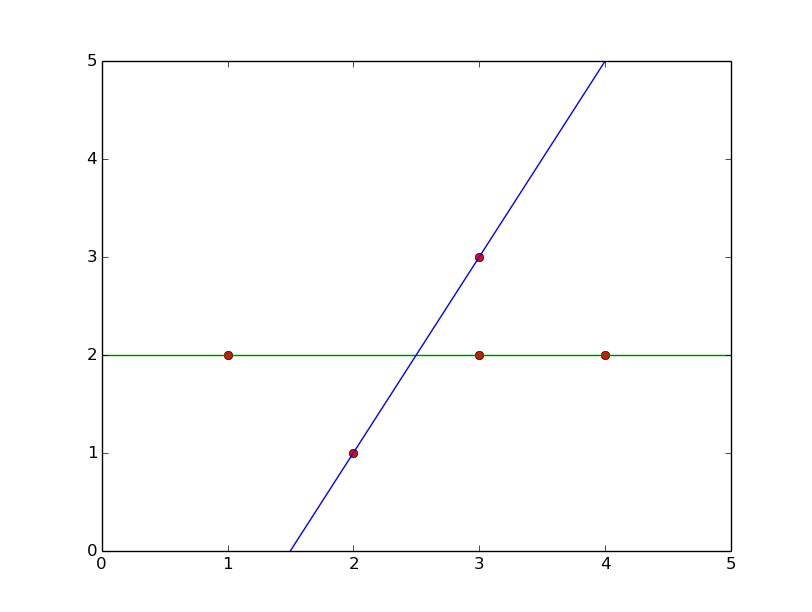
\includegraphics[width=7cm, height=6cm]{ejemploHame1}
  \caption{Puntos distribuidos inicialmente.}
\end{figure}

Una posible solución óptima sería lanzar 2 Kamehameha, 1 que mate a 3 androides (al 1, 3 y 4), la recta verde, y otro que mate a los otros 2, la recta azul.

\subsection{Descripción de la resolución}
La idea del algoritmo es que recursivamente vaya creando todas las combinaciones de rectas. Esto lo logramos utilizando una función principal, Kamehameha, a la que recurrimos y 2 funciones, una que se fija si un androide puede ser atacado con un Kamehameha ya lanzado (si esta alineado con algun con algun otro grupo de androides ya atacados) y vuelve a llamar a la función principal con los nuevos valores una vez por cada grupo con el que esta alineado este androide y otra función que comienza un nuevo ataque con ese androide y vuelve a llamar a la función principal. De esta forma, probando con un enemigo, volviendo atras, probando con el siguiente, volviendo atras y asi sucesivamente hasta probar con todos los enemigos, podemos generar todas las posibles combinaciones de líneas. Lo único que resta es verificar cual de estas es la óptima. Para conseguirlo, cada vez que generamos una solución completa, verificamos su tamaño (su acantidad de líneas) y la guardamos si es la menor hasta el momento, sino la descartamos.
Para mejorar el tiempo de ejecución decidimos agregar un a poda que descarta soluciones que estan siendo generadas en el momento que su tamaño supera el tamaño de la solución minima alamacenada, ya que sabemos que si o si es mayor o igual a la que ya tenemos, por lo tanto no nos sirve.

\subsection{Pseudocódigo}
\begin{verbatim}
\end{verbatim}

\subsection{Cota de complejidad}
\paragraph{Como ya explicamos, usamos recursividad y 2 funciones. En cada llamado recursivo usamos las 2 funciones. La que genera un nuevo ataque es O(1) ya que hace una cantidad acotada de operaciones O(1). La otra, verifica si un enemigo esta alineado con los otros una vez por cada ataque realizado hasta el momento. Lala cantidad de ataques es acotada, ya que como cualqueir par de puntos puede ser unido con una recta, la cantidad de ataques o rectas necesarios es menor o igual a $n/2$, siendo $n$ la cantidad total de enemigos. De esta forma vemos que esta función es O($n/2$).

}

\subsection{Extracto importante de código}
\begin{lstlisting}
typedef pair<int,int> posicion_t;
typedef vector<posicion_t> Kamehameha_t;
typedef vector<Kamehameha_t> Kamehamehas_t;
typedef deque<posicion_t> listaPos_t;

int minimo_global = std::numeric_limits<int>::max();
listaPos_t enemigos_global;
Kamehamehas_t mejor_configuracion;

void Kamehameha(listaPos_t enemigos,
                Kamehamehas_t enLaMira,
                int indexRectaActual);
void atacarEnAtaqueActual(posicion_t enemigo,
                          listaPos_t restoEnemigos,
                          Kamehamehas_t ataques,
                          int nroAtaque);
void atacarEnNuevoAtaque(posicion_t enemigo,
                         listaPos_t restoEnemigos,
                         Kamehamehas_t ataques,
                         int nroAtaque);
bool alineados (Kamehameha_t atacados, posicion_t enemigo);
void reporte(listaPos_t enemigos, Kamehamehas_t ataques, int nroAtaque);
int buscarPosicion(const posicion_t& enemigo);
void mostrarSolucion();

int main() {
    int cantEnemigos;
    cin >> cantEnemigos;
    listaPos_t enemigos;
    Kamehamehas_t enLaMira;
    Kamehameha_t kamehameha;
    enLaMira.push_back(kamehameha);
    int indexRectaActual;
	posicion_t posicion;
    srand(time(NULL));
    for (int i = 0; i < cantEnemigos; i++) {
        int x = rand() %10;
        int y = rand() %10;
    	posicion = make_pair(x, y);
    	enemigos.push_back((posicion));
    }
    //Para imprimir las tuplas generadas al azar:
    enemigos_global = enemigos;
    for (listaPos_t::iterator it = enemigos.begin(); it != enemigos.end(); ++it) {
            cout << (*it).first << " " << (*it).second << endl;
    }
    Kamehameha(enemigos, enLaMira, 0);
    mostrarSolucion();
    return 0;
}

void Kamehameha(listaPos_t enemigos, Kamehamehas_t ataques, int nroAtaque) {
    if (enemigos.size() == 0) {
        if (minimo_global > (int)ataques.size()) {
            minimo_global = (int) ataques.size();
            mejor_configuracion = ataques;
        }
    } else {
        for (int i = 0; i < enemigos.size(); i++) {
            posicion_t enemigo = enemigos.front();
            enemigos.pop_front();
            atacarEnAtaqueActual(enemigo, enemigos, ataques, nroAtaque);
            atacarEnNuevoAtaque(enemigo, enemigos, ataques, nroAtaque);
            enemigos.push_front(enemigo);
        }
    }
}

void atacarEnAtaqueActual(posicion_t enemigo, listaPos_t restoEnemigos, Kamehamehas_t ataques, int nroAtaque) {
    Kamehameha_t atacados = ataques[nroAtaque];
    if (atacados.size() == 0){
        Kamehameha_t comenzarAtaque;
        comenzarAtaque.push_back(enemigo);
        ataques[nroAtaque] = comenzarAtaque;
        Kamehameha(restoEnemigos, ataques, nroAtaque);
        Kamehameha_t reestablecerAtaque;
        ataques[nroAtaque] = reestablecerAtaque;
    } else if (alineados(atacados, enemigo)) {
        ataques[nroAtaque].push_back(enemigo);
        Kamehameha(restoEnemigos, ataques, nroAtaque);
        ataques[nroAtaque].pop_back();
    } else {
        return;
    }
}

void atacarEnNuevoAtaque(posicion_t enemigo, listaPos_t restoEnemigos, Kamehamehas_t ataques, int nroAtaque) {
    if (ataques[nroAtaque].size() > 0) {
        Kamehameha_t comenzarAtaque;
        comenzarAtaque.push_back(enemigo);
        ataques.push_back(comenzarAtaque);
        nroAtaque++;
        Kamehameha(restoEnemigos, ataques, nroAtaque);
        nroAtaque--;
        ataques.pop_back();
    }
}

bool alineados (Kamehameha_t atacados, posicion_t enemigo) {
    if (atacados.size() == 0 || atacados.size() == 1) {
        return true;
    } else {
        posicion_t primero = atacados[0];
        posicion_t segundo = atacados[1];
        int termino1 = segundo.second - primero.second;
        int termino2 = enemigo.first - primero.first;
        int termino3 = enemigo.second - primero.second;
        int termino4 = segundo.first - primero.first;
        return termino1*termino2 == termino3*termino4;
    }
}

void reporte(listaPos_t enemigos, Kamehamehas_t ataques, int nroAtaque) {
    cout << "enemigos: ";
    for (listaPos_t::iterator itL = enemigos.begin(); itL != enemigos.end(); ++itL) {
        cout << "(" << (*itL).first << ", " << (*itL).second << ")";
        if (itL!= enemigos.end()) {
            cout << ", ";
        }
    }
    cout << endl ;
    for (int i = 0; i < ataques.size(); i++) {
        Kamehameha_t ataqueEnIdx = ataques[i];
        cout << "[";
        for (Kamehameha_t::iterator it = ataqueEnIdx.begin(); it != ataqueEnIdx.end(); ++it) {
            cout << "(" << (*it).first << ", " << (*it).second << "), ";
            if (it!= ataqueEnIdx.end()){ cout << ", "; };
        }
        cout << "]" << endl;
    }
}

void mostrarSolucion() {
    cout << mejor_configuracion.size() << endl;
    for (int i = 0; i < mejor_configuracion.size(); i++) {
        Kamehameha_t ataqueEnIdx = mejor_configuracion[i];
        cout << ataqueEnIdx.size() << " ";
        for (Kamehameha_t::iterator it = ataqueEnIdx.begin(); it != ataqueEnIdx.end(); ++it) {
            cout << (buscarPosicion(*it)+1) << " ";
        }
        cout << endl;
    }
}

int buscarPosicion(const posicion_t& enemigo) {
    listaPos_t::iterator it = find (enemigos_global.begin(), enemigos_global.end(), enemigo);
    return distance(enemigos_global.begin(), it);
}
\end{lstlisting}

\subsection{Experimentacion}
\begin{verbatim}
Se puede observar que el tiempo que tarda el algoritmo es relativo a la distribucion de los puntos, aunque principalmente a la cantidad que sean. A partir de 16 puntos el algoritmo tarda mas de un minuto.

Cantidad de puntos = 1
Posiciones = 9 8
El tiempo que tardo es:1.7e-05
Rectas que necesitamos = 1
1 1 

Cantidad de puntos = 2
Posiciones = 12 5 - 9 3
El tiempo que tardo es:3.2e-05
Rectas que necesitamos = 1
2 1 2 
   
Cantidad de puntos = 3
Posiciones = 6 3 - 14 7 - 3 12
El tiempo que tardo es:4.4e-05
Rectas que necesitamos = 2
2 1 2 
1 3 
   
Cantidad de puntos = 4
Posiciones = 13 0 - 1 12 - 9 10 - 10 1
El tiempo que tardo es:6e-05
Rectas que necesitamos = 2
2 1 2 
2 3 4 
   
Cantidad de puntos = 5
Posiciones = 9 0 - 11 6 - 14 12 - 12 8 - 5 9
El tiempo que tardo es:0.000175
Rectas que necesitamos = 2
2 1 5 
3 2 3 4 
   
Cantidad de puntos = 6
Posiciones = 5 4 - 0 11 - 1 7 - 3 9 - 10 10 - 12 3
El tiempo que tardo es:0.000169
Rectas que necesitamos = 3
2 1 2 
2 3 4 
2 5 6 
   
Cantidad de puntos = 7
Posiciones = 12 9 - 7 13 - 5 10 - 10 14 - 9 7 - 0 3 - 11 8
El tiempo que tardo es:0.000836
Rectas que necesitamos = 4
2 1 2 
2 3 4 
2 5 6 
1 7 
   
Cantidad de puntos = 8
Posiciones = 6 13 - 7 3 - 1 0 - 4 10 - 8 6 - 3 9 - 0 5 - 12 2
El tiempo que tardo es:0.00056
Rectas que necesitamos = 3
3 1 6 7 
2 2 3 
3 4 5 8 
   
Cantidad de puntos = 9
Posiciones = 7 11 - 12 2 - 8 0 - 0 3 - 13 12 - 6 5 - 1 7 - 3 6 - 9 1
El tiempo que tardo es:0.006745
Rectas que necesitamos = 5
2 1 2 
2 3 4 
2 5 6 
2 7 8 
1 9 
   
Cantidad de puntos = 10
Posiciones = 6 9 - 4 12 - 2 14 - 8 7 - 3 3 - 9 10 - 5 4 - 11 6 - 10 13 - 14 2
El tiempo que tardo es:0.002715
Rectas que necesitamos = 4
2 1 5 
3 2 3 10 
3 4 6 9 
2 7 8 
   
Cantidad de puntos = 15
Posiciones = 0 2 - 5 5 - 14 8 - 3 13 - 9 4 - 7 14 - 8 12 - 12 1 - 10 11 - 6 3 - 4 9 - 13 7 - 11 6 - 2 0 - 1 10
El tiempo que tardo es:0.785094
Rectas que necesitamos = 7
2 1 2 
2 3 4 
2 5 6 
2 7 10 
3 8 9 13 
2 11 12 
2 14 15 

Gafico que representa este experimento:

\end{verbatim}

\end{document}
